\setlength{\columnsep}{3pt}
\begin{flushleft}

\bigskip
\textbf{What is a network?}
\newline
A network \textbf{consists of two or more computers that are linked in order to share resources (such as printers and CDs)}, exchange files, or allow electronic communications.

\begin{figure}[h!]
	\centering
	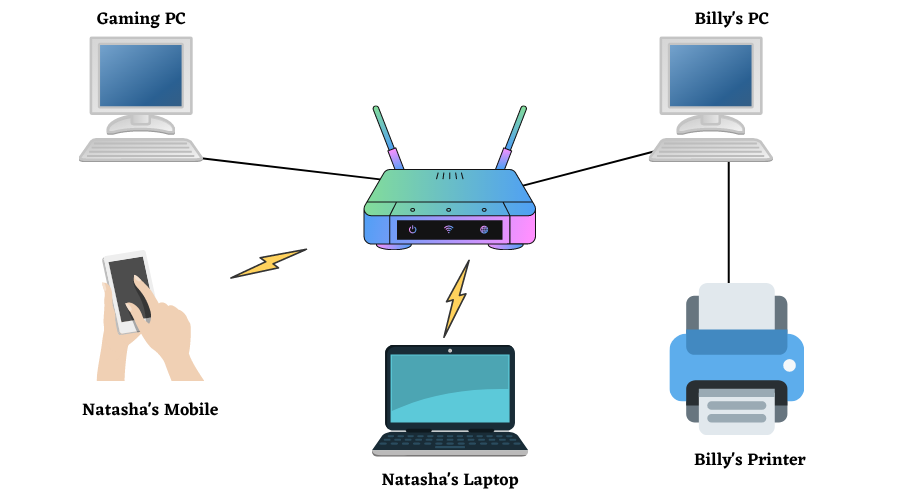
\includegraphics[scale=0.6]{content/chapter14/images/networking.png}
	\caption{Network of device}
	\label{fig:network}
\end{figure}

\newpage

\textbf{Let's see the types of network available:}

\begin{figure}[h!]
	\centering
	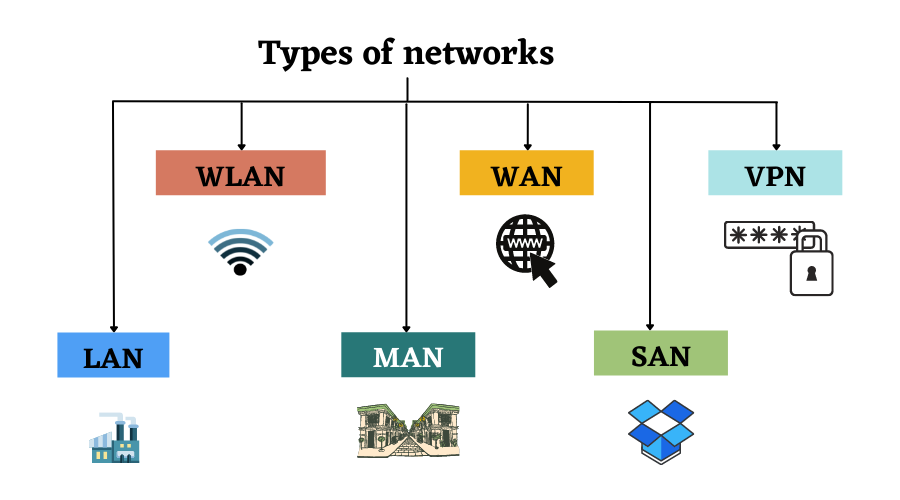
\includegraphics[scale=0.6]{content/chapter14/images/network_types.png}
\end{figure}

\begin{itemize}
	\item \textbf{Local Area Network (LAN)}:
	\begin{itemize}
		\item \textbf{Connect computers across short distances}(like group of buildings close to each other) to share information/resources.
		\item \textbf{Companies uses LANs}.
	\end{itemize}
	\bigskip\bigskip
	\item \textbf{Wireless Local Area Network (WLAN)}:
	\begin{itemize}
		\item Functions like a LAN.
		\item WLANs make use of wireless network technology, such as Wi-Fi.
	\end{itemize}
	\bigskip\bigskip
		\item \textbf{Wide Area Network (WAN)}:
	\begin{itemize}
		\item Connects computers together across longer physical distances.
		\item Eg: The Internet
		\item Maintained by multiple administrators or the public.
	\end{itemize}
	\bigskip\bigskip
	\item \textbf{Metropolitan Area Network (MAN)}:
	\begin{itemize}
		\item Larger than LANs but smaller than WANs.
		\item Span an \textbf{entire geographic area} (eg. town or city).
		\item Handled by single person or company.
	\end{itemize}
	\bigskip\bigskip
	\item \textbf{Storage-Area Network (SAN)}:
	\begin{itemize}
		\item \textbf{Connects shared pools of storage devices to several servers}.
		\item \textbf{SAN doesn't rely on a LAN or WAN}.
		\item Storage resources are placed into high-performance network.
	\end{itemize}
	\bigskip\bigskip
	\item \textbf{Virtual Private Network (VPN)}:
	\begin{itemize}
		\item \textbf{Private network across the Internet}.
		\item Lets its users send and receive data over private network using Internet.
	\end{itemize}



\end{itemize}


\end{flushleft}
\newpage


